%%%%%%%%%%%%%%%%%%%%%%%%%%%%%%%%%%%%%%%%%%%%%%%%%%%%%%%%%%%%%%%%%%%%%%
% amspaper.tex --  LaTeX2e-based template for submissions to American 
% Meteorological Society Journals, including
%
% JAS 	-- Journal of the Atmospheric Sciences
% JAMC 	-- Journal of Applied Meteorology and Climatology
% JPO 	-- Journal of Physical Oceanography
% MWR 	-- Monthly Weather Review
% JTECH -- Journal of Atmospheric and Oceanic Technology
% WAF 	-- Weather and Forecasting
% JCLI 	-- Journal of Climate
% JHM 	-- Journal of Hydrometeorology
% JAM 	-- Journal of Applied Meteorology
%
% Template developed by B. Papa and S. Cooley, AMS. 
% Email questions to latex@ametsoc.org.
%
% August 12, 2008 (SRC)
%	- Clarified/added header notes, comments throughout
%	- Improved title page
%	- Edited text of document for clarity
%	- Altered list styles to adhere to AMS style, added comments
%	- Removed incorrect commands (i.e., \catcode) (corrects umlaut bug)
%	- Moved non-template commands to ametsoc.sty
%
% August, 2008 - B. Papa
% - Updated to handle two column journal page output
% - Updated text with new/modified instructions
%
%%%%%%%%%%%%%%%%%%%%%%%%%%%%%%%%%%%%%%%%%%%%%%%%%%%%%%%%%%%%%%%%     
%%%%%%%%%%%%%%%%%%%%%%%%%%%%%%%%%%%%%%%%%%%%%%%%%%%%%%%%%%%%%%%%
%																															 %
%				USE THIS TEMPLATE, AMETSOC.STY, AND AMETSOC.BST				 %
%			        OR YOUR TEX FILES WILL NOT BE USED				  		 %
%																															 % 
%%%%%%%%%%%%%%%%%%%%%%%%%%%%%%%%%%%%%%%%%%%%%%%%%%%%%%%%%%%%%%%%
%%%%%%%%%%%%%%%%%%%%%%%%%%%%%%%%%%%%%%%%%%%%%%%%%%%%%%%%%%%%%%%%

%%%%%%%%%%%%%%%%%%%%%%%%%%%%%%%%%%%%%%%%%%%%%%%%%%%%%%%%%%%%%%%%%%%%%
% PREAMBLE
%%%%%%%%%%%%%%%%%%%%%%%%%%%%%%%%%%%%%%%%%%%%%%%%%%%%%%%%%%%%%%%%%%%%%
%
% The following two commands will generate a PDF that follows all the requirements for submission
% and peer review.  Uncomment these commands to generate this output (and comment out the two lines below.)
%
% DOUBLE SPACE VERSION FOR SUBMISSION TO THE AMS
\documentclass[12pt]{article}
\usepackage{ametsoc}
\linenumbers
%
% The following two commands will generate a single space, double column paper that closely
% matches an AMS journal page.  Uncomment these commands to generate this output (and comment
% out the two lines above. FOR AUTHOR USE ONLY. PAPERS SUBMITTED IN THIS FORMAT WILL BE RETURNED
% TO THE AUTHOR for submission with the correct formatting.
%
% TWO COLUMN JOURNAL PAGE LAYOUT FOR AUTHOR USE ONLY
%\documentclass[10pt]{article}
%\usepackage{ametsoc2col}
\usepackage{subfigure}
\usepackage{comment}
\usepackage{verbatim}
\usepackage{fancyvrb}

%
%%%%%%%%%%%%%%%%%%%%%%%%%%%%%%%%%%%%%%%%%%%%%%%%%%%%%%%%%%%%%%%%%%%%%
% ABSTRACT
%
% Enter your Abstract here
%%%%%%%%%%%%%%%%%%%%%%%%%%%%%%%%%%%%%%%%%%%%%%%%%%%%%%%%%%%%%%%%%%%%%
\newcommand{\myabstract}{Several strategies are designed and implemented in the data assimilation system for the Weather Research and Forecasting model to parallel assimilate the global positioning system (GPS) radio occultation (RO) sounding with the nonlocal excess phase delay operator, which is computational expensive and has been proven to produce significantly better analysis for numerical weather predictions compared to local refractivity operator. In particular, to solve the parallel load imbalance problem due to the uneven geographic distribution of the GPS RO observations, the round-robin scheduling is adopted to distribute GPS RO observations to balance the workload among the processing cores. The wallclock time required to complete $5$ iterations of minimization on a demonstration Antarctic case with $106$ GPS RO observations, is reduced from more than $3.5$ hours with single processor to $2.5$ minutes with $106$ processing cores. These strategies present the possibility of the application of the nonlocal GPS excess phase delay operator in the operational data assimilation systems with a cut-off time limit.}
%
\begin{document}
%
%%%%%%%%%%%%%%%%%%%%%%%%%%%%%%%%%%%%%%%%%%%%%%%%%%%%%%%%%%%%%%%%%%%%%
% TITLE
%
% Enter your TITLE here
%%%%%%%%%%%%%%%%%%%%%%%%%%%%%%%%%%%%%%%%%%%%%%%%%%%%%%%%%%%%%%%%%%%%%
\title{\textbf{\large{Parallel Strategies for the GPS Radio Occultation Data Assimilation with a Nonlocal Operator in the Weather Research and Forecasting model}}}
%
% Author names, with corresponding author information. 
% [Update and move the \thanks{...} block as appropriate.]
%
\author{\textsc{Xin Zhang}
				\thanks{\textit{Corresponding author address:} 
				Dr. Xin Zhang, NCAR, MMM, P.O. Box 3000, 
				 Boulder, CO 80307. 
				\newline{E-mail: xinzhang@ucar.edu}}\\
\textit{\footnotesize{National Center for Atmospheric Research, Boulder, Colorado 80307, USA}}
\and 
\centerline{\textsc{Ying-Hwa Kuo}}\\% Add additional authors, different institution
\centerline{\textit{\footnotesize{National Center for Atmospheric Research, Boulder, Colorado 80307, USA}}}
\and 
\centerline{\textsc{Shu-Ya Chen}}\\% Add additional authors, different institution
\centerline{\textit{\footnotesize{National Center for Atmospheric Research, Boulder, Colorado 80307, USA}}}
\and 
\centerline{\textsc{Xiang-Yu Huang}}\\% Add additional authors, different institution
\centerline{\textit{\footnotesize{National Center for Atmospheric Research, Boulder, Colorado 80307, USA}}}
\and
\centerline{\textsc{Ling-Feng Hsiao}}\\% Add additional authors, different institution
\centerline{\textit{\footnotesize{Taiwan Typhoon and Flood Research Institute, Taipei, Taiwan}}}
}
%
% The following block of code will handle the formatting of the title page depending on whether
% we are formatting a double column (dc) author draft or a single column paper for submission.
% AUTHORS SHOULD SKIP OVER THIS... There is nothing to do in this section of code.
\ifthenelse{\boolean{dc}}
{
\twocolumn[
\begin{@twocolumnfalse}
\amstitle

% Start Abstract (Enter your Abstract above.  Do not enter any text here)
\begin{center}
\begin{minipage}{13.0cm}
\begin{abstract}
	\myabstract
	\newline
	\begin{center}
		\rule{38mm}{0.2mm}
	\end{center}
\end{abstract}
\end{minipage}
\end{center}
\end{@twocolumnfalse}
]
}
{
\amstitle
\begin{abstract}
\myabstract
\end{abstract}
\newpage
}
%%%%%%%%%%%%%%%%%%%%%%%%%%%%%%%%%%%%%%%%%%%%%%%%%%%%%%%%%%%%%%%%%%%%%
% MAIN BODY OF PAPER
%%%%%%%%%%%%%%%%%%%%%%%%%%%%%%%%%%%%%%%%%%%%%%%%%%%%%%%%%%%%%%%%%%%%%
%
\section{Introduction}

The observations from the global positioning system (GPS) radio occultation (RO) limb sounding technique has been proven as a valuable observation of atmosphere for numerical weather prediction (NWP) and climate research (\cite{Kuo1997}; \cite{ZouGPS1999}; \cite{zouGPS2000}; \cite{LiuandZou2003}; \cite{Healy2005}; \cite{HuangCY2005}; \cite{Cucurull2006}; \cite{Cucurull2008}; \cite{Healy2006}). GPS RO data has several advantages such as a high vertical resolution, no need for calibration, unaffected by cloud cover and rainfall, and global coverage. In particular, in the middle of upper troposphere, the GPS RO measurements have accuracy comparable with or better than that of radiosondes (\cite{Kuo2005}). Since the launch of the Constellation Observing System for Meteorology, Ionosphere, and Climate (COSMIC) mission in 2006, approximately ${\sim}$1500-2500 globally distributed GPS RO sounding are provided per day in near-real time. The COSMIC GPS RO sounding are currently being used at several global operational NWP centers, including the National Centers for Environmental Prediction (NCEP; \cite{Cucurull2008}), the European Centre for Medium-Range Weather Forecasts (ECMWF; \cite{Healy2008}), the Met Office (UKMO), and M\'et\'eo France (\cite{Poli2009}).

Due to the success of COSMIC, U.S. agencies and Taiwan have decided to move forward with a follow-on RO mission (called FORMOSAT-7/COSMIC-2) that will launch six satellites into low-inclination orbits in late 2015, and another six satellites into high-inclination orbits in early 2018. The COSMIC-2 mission will provide nearly an order of magnitude more RO data increase in the number of atmospheric and ionospheric observations that will greatly benefit the research and operational communities (http://www.cosmic.ucar.edu/cosmic2/).

Depending on the level of data processing, various variables can be retrieved from GPS RO observations for use in data assimilation, such as bending angel, refractivity and retrieved moisture/temperature profile ( See  \cite{Kuo2000}, \cite{Kuo2004}). To account for the variations of the atmospheric states along the GPS ray paths, the nonlocal excess phase operator, introduced by \cite{Soko2005}, has proven to significantly improve the assimilation of GPS RO data (\cite{Soko2005}, \cite{Liu2008}, \cite{ChenSY2009}, \cite{Ma2009} and \cite{Shao2009}). However, due to the high computational cost associated with the nonlocal operator, it has been tested only in some research configurations with affordable number of observations. The parallel implementation of the GPS RO data assimilation with nonlocal operator is urgently needed to advance its applications in both research and operational data assimilation systems. 

Because both the local refractivity and nonlocal excess phase delay operators had been implemented in the data assimilation system for Weather Research and Forecasting model (WRFDA, \cite{Barker2012}, \cite{ChenSY2009}), the three-dimensional variational (3D-Var) approach in WRFDA will be used throughout this paper to demonstrate the parallelization of GPS nonlocal operator. We believe that the parallel strategies for nonlocal operator are general and applicable for other parallel data assimilation systems (such as four-dimensional variational, and Ensemble Kalman Filter) employing the domain-decomposition approach.

This article is organized as follows. In Section \ref{sec:operators}, we briefly introduce both the local refractivity operator and nonlocal excess phase delay operators implemented in WRFDA and their computational costs. Section \ref{sec:strategy} provides the technical details of how the nonlocal GPS RO operator is paralleled in a domain-decomposition parallel context. The strategy to solve the load imbalance problem is presented in Section \ref{sec:load}. Sec. \ref{sec:opt} presents some further optimization to save the cost. The summary and discussion are given in Section \ref{sec:end}.
%%%%%%%%%%%%%%%%%%%%%%%%%%%%%%%%%%%%%%%%%%%%%%%%%%
\section{Local and Nonlocal GPS RO Operators}
\label{sec:operators}
In both local and nonlocal GPS RO operators, the neutral atmospheric refractivity can be calculated from model variables via the following relationship
\begin{equation}
\label{ref}
N = 77.6\frac{P}{T} + 3.73\times10^5\frac{P Q}{T^2(0.622+0.378Q)}
\end{equation}
where $P$ is the total atmospheric pressure in $hPa$; $T$ is the atmospheric temperature in $K$; and $Q$ is the specific humidity in ${kg}/{kg}$. The local GPS RO refractivity operator assumes that the observed refractivity is modeled as the local refractivity at the perigee point where the GPS ray is closest to the earth. The first guess fields of $P$, $T$ and $Q$ are interpolated horizontally and vertically to the perigee point of the RO observation and the Eqs. (\ref{ref}) is used to calculate the local refractivity. The local GPS RO refractivity operator is simple and low computational cost, and it is used by most of the data assimilation systems. 

To account for the variations of the atmospheric states along the GPS ray paths, the nonlocal excess phase operator, introduced by \cite{Soko2005}, simulates the excess phase by integrating the local refractivity along the ray path, which is approximated by a straight line. The new observation $S$ (excess phase, which is to be assimilated) is defined as
 \begin{equation}
 \label{excess}
 S = \int_{ray} N\; \mathrm{d}l
  \end{equation}
  where $l$ is the ray path and $N$ is the refractivity. There are two steps associated with the implementation of the nonlocal operator (\cite{ChenSY2009}, \citet{Ma2009}, and \cite{Liu2008}): Firstly, the observed excess phase is calculated by integrating the refractivity from RO observations:
  \begin{equation}
  \label{excess-o}
  S_{obs} = \int_{ray} N_{RO}(r)\; \mathrm{d}l
  \end{equation}
  where $r$ is the radius vector derived from $r=r_c+z$, $r_c$ is the local curvature radius of the earth, and $z$ is the height above the earth's surface, $N_{RO}$ is the observed refractivity interpolated on the model mean heights of the tangent point position by a vertical average. The next step is to calculate the model counterpart $S_{mod}$, which is given by
 \begin{equation}
 \label{excess-m}
 S_{mod} = \int_{ray} N_{mod}(r)\; \mathrm{d}l
 \end{equation}
where  $N_{mod}$ is the simulated refractivity from first guess fields of $T$, $P$, and $Q$ by Eqs. (\ref{ref}) and interpolated at the tangent point position. 

Compared to the local GPS refractivity operator, the computational cost of the nonlocal excess phase operator is increased dramatically due to the integration of refractivity along the GPS ray. \cite{Liu2008} reports that the cost of nonlocal to local operator is at least $100$ times on a Linux cluster of NCAR. To justify the necessity to parallel the GPS RO nonlocal operator, an Antarctic domain with $30km$ horizontal resolution, shown as Fig. \ref{domain}, is chosen to demonstrate the computational cost of the GPS RO operators. This is a Advanced Research WRF (\cite{Skamarock2008}) model domain of 1800 UTC 11 December 2007 with $401\times401$ mesh size and 55 vertical layers between surface and $10$ $hPa$. Fig. \ref{domain} also shows the locations of the $106$ GPS RO profiles within $\pm3$ hours window centered at 1800UTC. The $106$ GPS RO profiles are assimilated with WRFDA 3D-Var on National Center for Atmospheric Research (NCAR)'s supercomputer yellowstone (http://www2.cisl.ucar.edu/resources/yellowstone) and the wallclock time of 5 iterations of minimization are recorded to demonstrate the computational costs. After excluding the program initialization and I/O, with single processing core, it takes only $146s$ to assimilate $106$ GPS RO profiles by local operator. However, about $12,762s$ ($\approx$ 3.5 hours) are needed to run 5 iterations with nonlocal operator. The ratio of the computational cost of nonlocal to local operator is about 87 for this case. In terms of the production 3D-Var run with 60 iterations (assumes 2 outer loops) approximately, the wallclock time for serially running this case will be more than 42 hours on yellowstone. Therefore, the cost of nonlocal operator with single processing core is extremely unaffordable for either research or operational purposes.

%%%%%%%%%%%%%%%%%%%%%%%%%%%%%%%%%%%%%%%%%%%%%%%%%%
\section{Parallelization Strategy}
\label{sec:strategy}
Most of the atmospheric models and their data assimilation systems employ the horizontal domain-decomposition method for parallel processing. In data assimilation systems, the observation is usually assigned to the subdomain where it is geographically located. However, for such as satellite radiance data assimilation, due to the uneven distribution of the observations and the expensive radiative transfer model, the radiance operator is expensive and the load imbalance issue has to be considered for operational practice. We may either change the way of the horizontal domain-decomposition method to have each subdomain cover similar number of radiance data, or redistribute the radiance data among processing cores to have each core has similar workload. Please note that the load balance algorithm itself might be costly and complicated.

The difficulty to parallel the nonlocal operator under the domain-decomposition context roots in its nonlocal integral nature of Eq. (\ref{excess-m}) along the ray-paths at all vertical levels above the tangent point and below the model top. The ray-path might intercepts several subdomains located on different processing cores respectively and each processing core is only aware of the atmospheric states of the local subdomain. Apparently, the most suitable strategy to parallel nonlocal GPS RO operator is the ray-path-wise distribution among processing cores (\cite{ZhangX2004}), which distributes the workload among processing cores based upon the number of the GPS ray-paths, instead of the geographic location of the observations. However, in our parallelization strategy, we must consider the fact of the existed domain-decomposition method to minimize the implementation cost. 

Although Eq. (\ref{excess-m}) is an integration of the refractivity along the ray-path, which might go through the whole model domain, we noticed that only one derived variable -- model simulated refractivity ($N_{mod}$) is used for the integration. If each processing core (subdomain) is aware of the global $N_{mod}$, the integration is able to be done on each whole ray-path parallel. The calculate of $N_{mod}$ from firstguess fields with Eq. (\ref{ref}) is trivial and each processing core can calculate the $N_{mod}$ of subdomain locally in advance. It turns out that we can use the parallel collecting-and-broadcasting operation to collect the local calculated $N_{mod}$ from each subdomain to a global $N_{mod}$ array and to broadcast the global $N_{mod}$ to each processing core. The costs for this strategy is the additional memory storage for several global arrays and the collecting-and-broadcasting operation in each iteration. For modern distributed memory supercomputers, the costs are trivial.

With the implementation of above parallel strategy (experiment "Parallel") , Fig. \ref{timing}(a) shows the parallel wallclock timing results with up to 512 processing cores on NCAR's yellowstone (red bars represent experiment "Parallel"). The wallclock time of 5 iterations minimization reduced from around $3.5$ hours with serial run to $279$ ($\approx$ 4.5 minutes) seconds with 512 processing cores. 

%%%%%%%%%%%%%%%%%%%%%%%%%%%%%%%%%%%%%%%%%%%%%%%%%%
\section{Load Balance}
\label{sec:load}
Fig. \ref{spd} shows the parallel speedups, which are the ratio of the wallclock times of parallel runs against that of the serial run. The black line is the linear parallel speedup and represents the ideal speedup or acceleration when multiple processing cores are used. The red line represents experiment "Parallel". The speedup with $512$ processing cores is $46$ and one may argue that  the actual speedup is much lower than the ideal speedup ($512$) and the parallelization strategy is not cost-effective. Therefore, the analysis of the parallel algorithm of the GPS RO operator will be helpful to understand the unsatisfactory speedup and identify the reason behind.

In Sec. \ref{sec:strategy}, we emphasized that we have to consider the existed horizontal domain-decomposition method for the GPS RO data distribution, which indicates that each GPS RO profile is assigned to the connected subdomain based on its geographic location. The location of the GPS RO profile is not fixed and changes for every occultation. The geographic distribution of GPS RO profiles is not even  (see Fig. \ref{domain}). Since the nonlocal excess phase operator for GPS RO data is very expensive and it is very likely that some processing cores or subdomains get more GPS RO profiles than others. One may deduce that the overall performance is solely determined by the workload of the processing cores which being assigned the most number of profiles to process. Fig. \ref{timing}(b) shows the variation of the maximum number of assigned observations per subdomain with the numbers of processing cores (red bars represent experiment "Parallel"). Because the uneven geographic distribution of the GPS RO profiles, even we used $512$ processing cores, there is still one out of $512$ subdomains covers two GPS RO profiles and most of the processing cores are idle. Therefore, the theoretic speedup with $512$ processing cores is $106/2=53$ and the actual speedup of $46$ should be considered as efficient enough for this strategy. It is impossible to achieve the ideal speedup before solving the load imbalance issue. Visual comparison of (a) and (b) in Fig. \ref{timing} for experiment "Parallel" suggests that the parallel performance has a very high correlation with the maximum number of the observation per processing core/subdomain. The load imbalance is the bottleneck of the overall parallel performance.

We have indicated in Sec. \ref{sec:strategy} that the most suitable parallel strategy for the nonlocal GPS RO operator is the ray-path-wise distribution. Taking advantage of the parallel strategy implemented in Sec. \ref{sec:strategy}, each processing core is aware of the global $N_{mod}$, which means that each processing core can calculate the integral of Eq. \ref{excess-m} along any ray-path of any profile. Therefore, it is feasible to distribute the GPS RO data ray-by-ray among processing cores in a round-robin fashion. However, taking into account the cost of implementation, it is much easier to distribute the GPS RO data profile-by-profile among processing cores in terms of the amount of code modification. Please note that since different GPS RO profile may includes different number of GPS ray-paths at vertical levels above the tangent point and below the model top, the profile-by-profile distribution may sacrifice some of the load balance compared to the ray-by-ray distribution. 

The experiment "Loadbalance" in Fig. \ref{timing}(a) shows the wallclock time spent with the number of processing cores up to $128$. Actually, $106$ is the minimum number of processing cores for this case to get the maximum theoretic parallel efficiency since we have $106$ GPS RO profiles.  With the round-robin distribution of the GPS RO profiles, each processing core is assigned with approximately equal number of the profiles. With $128$ processing cores, the wallclock time is reduced to $162$ ($\approx$ 2.5 minutes) seconds for 5 iterations minimization including initialization and I/O. Compared to $492$ seconds with $128$ processing cores and $279$ seconds with $512$ processing cores in Sec. \ref{sec:strategy}, the load balance strategy tremendously increases the parallel efficiency of the nonlocal excess phase GPS RO operator. The experiment "Loadbalance" in Fig. \ref{spd} shows that the speedup with $128$ processing cores is $80$. More precisely speaking, the speedup with $106$ processing core is $80$. Without the load balance strategy, the speedup with $128$ processing cores is $33$. Again, the high correlation between the wallclock times and the maximum number of observations per processing cores of experiment "Loadbalance" in (a) and (b) of Fig. \ref{timing} confirms the analysis that the importance of the load balance strategy in parallel data assimilation of GPS RO data with nonlocal operator.

%%%%%%%%%%%%%%%%%%%%%%%%%%%%%%%%%%%%%%%%%%%%%%%%%%
\section{Further Optimization}
\label{sec:opt}
In variational data assimilation methods, not only the observation operator is needed to calculate the innovation, but also the corresponding tangent linear and adjoint observation operators are required during the minimization. The tangent linear and adjoint operators are used to evolve the perturbations forward and backward along the basic trajectory, respectively. Therefore, it is an economic way to save the computational cost if the basic trajectory could be recorded, other than recomputed. In terms of the nonlocal GPS RO operator implementation in the WRFDA system (\cite{ChenSY2009}), the locations of each ray-path should be recored during the innovation calculation and the recorded location of each ray-path can be used in tangent linear adjoint operators directly. The experiment "Optimization" in Fig. \ref{timing}(a) shows the wallclock timing results with this further optimization. Averaged $4\% \sim 10\%$ further acceleration is observed.

%%%%%%%%%%%%%%%%%%%%%%%%%%%%%%%%%%%%%%%%%%%%%%%%%%
\section{Summary and Discussion}
\label{sec:end}
The nonlocal excess phase operator for GPS RO data has been demonstrated to be a solid and promising method to simulate the the observed GPS excess phase delay from the model states. However, due to its high computational cost and the nonlocal nature in the algorithm which includes the integration along the GPS ray-path across the model domain, it is not easy to implement this new operator in data assimilation systems parallelized based on the horizontal domain-decomposition method. Therefore, it has been tested only in some research configurations with affordable number of observations.

To parallel the nonlocal excess phase GPS RO operator, the first strategy is to enable each processing core to be aware of the global simulated model refractivity, which is the only variable needed for the nonlocal operator and is calculated in advance. Thus, each processing core can process the GPS observations geographically located within its connected subdomain. However, the performance analysis reveals that the load imbalance associated with the default geographic observation distribution among processing cores seriously constrains the parallel efficiency. Leveraging the implementation of the first strategy, GPS RO profiles can be alternatively distributed among processing cores in a round-robin fashion, which ensures the best possible load balance with available computing resource. The demonstration case with $106$ GPS RO profiles over a Antarctic domain shows that the wallclock time for 5 iterations minimization with WRFDA reduced from about 3.5 hours with one processing core to approximately 2.5 minutes with $106$ processing cores. This is affordable in terms of both research and operational practices.

Depends on the height of tangent point of the GPS occultation, different GPS RO profiles may has different number of levels, therefore, different number of ray-paths. As mentioned before, better load balance and further acceleration is still possible if the GPS RO data is distributed among processing cores ray-by-ray. However, the ray-path has to be determined before the data distribution and this may include some substantial code changes.


\section{Figures and tables}

\subsection{Figures}

%%%%%%%%%%%%%%%%%%%%%%%%%%%%%%%%%%%%%%%%%%%%%%%%%%%%%%%%%%%%%%%%%%%%%
% FIGURES
%%%%%%%%%%%%%%%%%%%%%%%%%%%%%%%%%%%%%%%%%%%%%%%%%%%%%%%%%%%%%%%%%%%%%
\begin{figure}
\noindent\includegraphics[width=20pc]{figures/obsloc2007121118.eps}
\caption{Experiment domain and the locations of $106$ GPS RO profiles (blue dots) within $\pm3$ hours of 1800 UTC 11 December 2007}
\label{domain}
\end{figure}
%
\begin{figure}
\noindent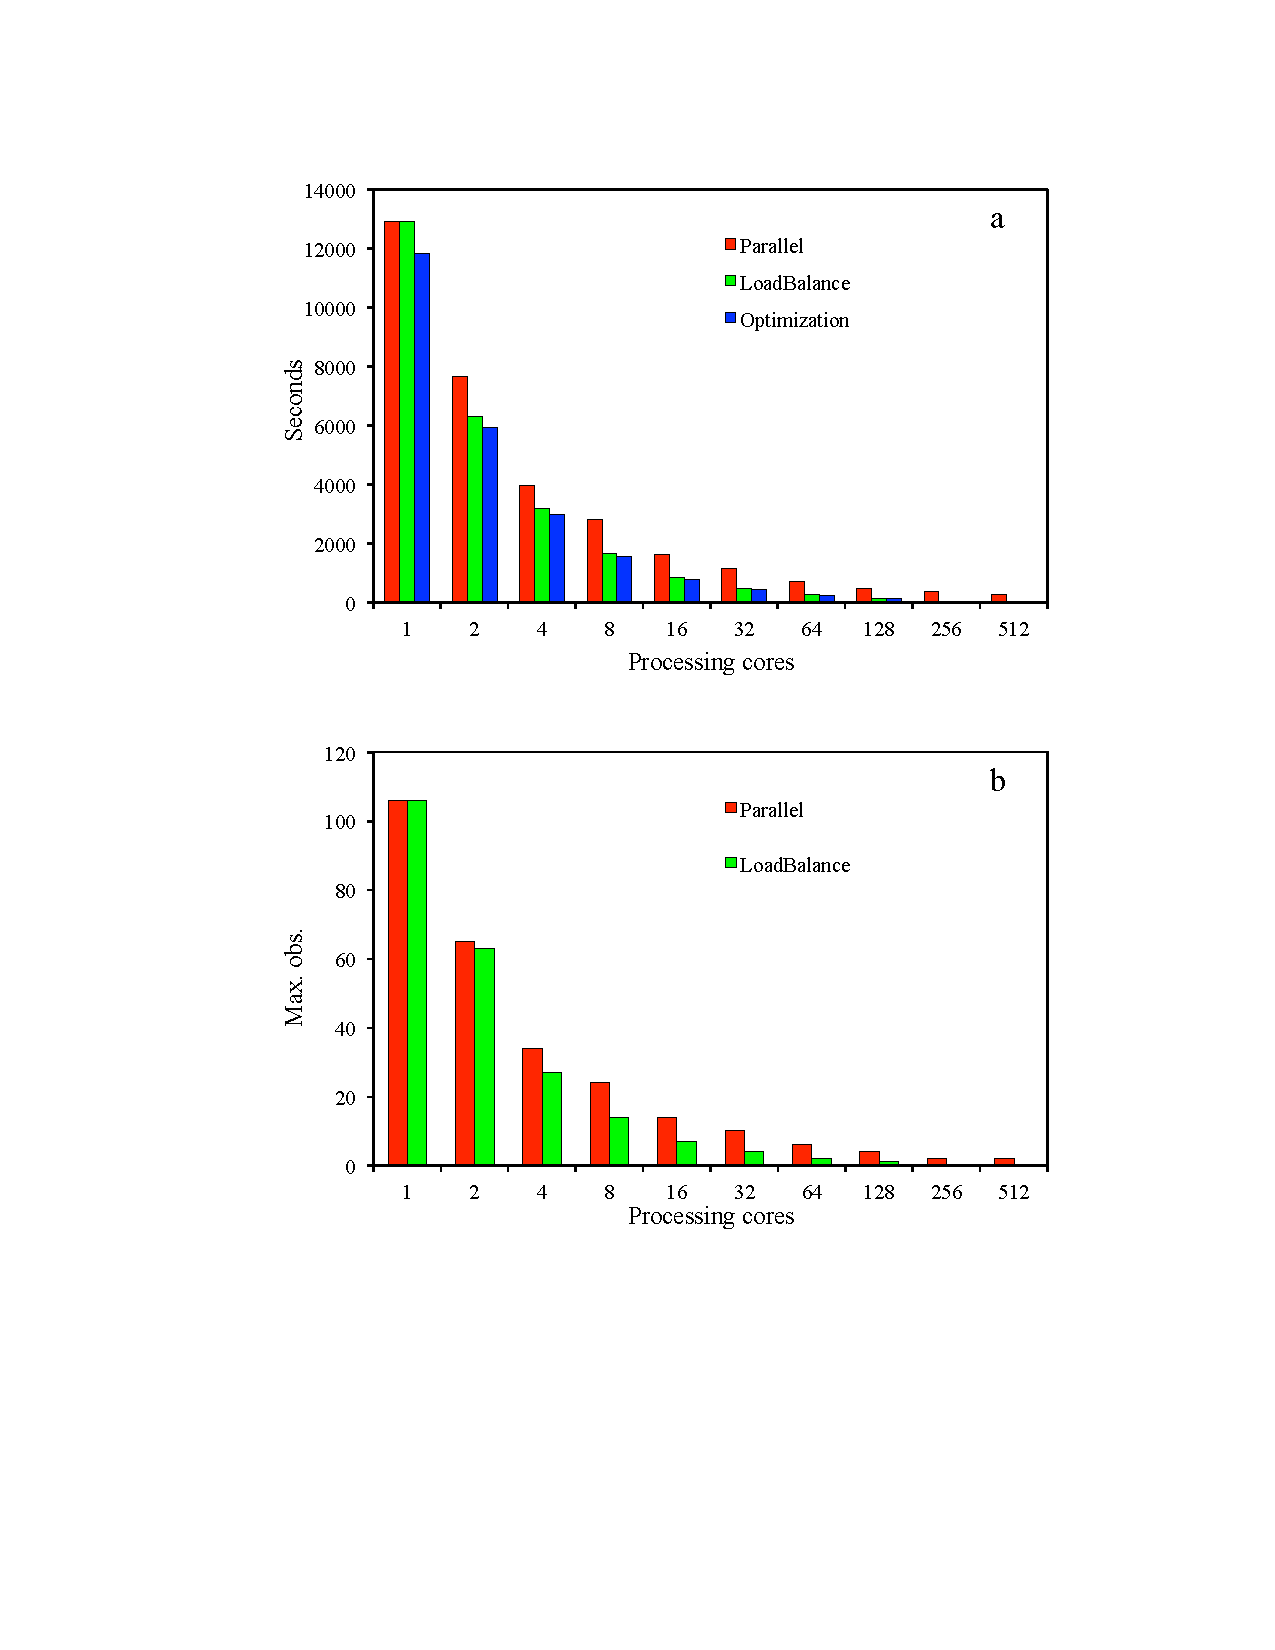
\includegraphics[width=40pc, trim=30 200 100 50, clip]{figures/Walltime.pdf}
\caption{The wallclock times (a) and maximum number of observation per processing core (b) for 5 iterations of minimization on NCAR yellowstone.}
\label{timing}
\end{figure}
%
\begin{figure}
\noindent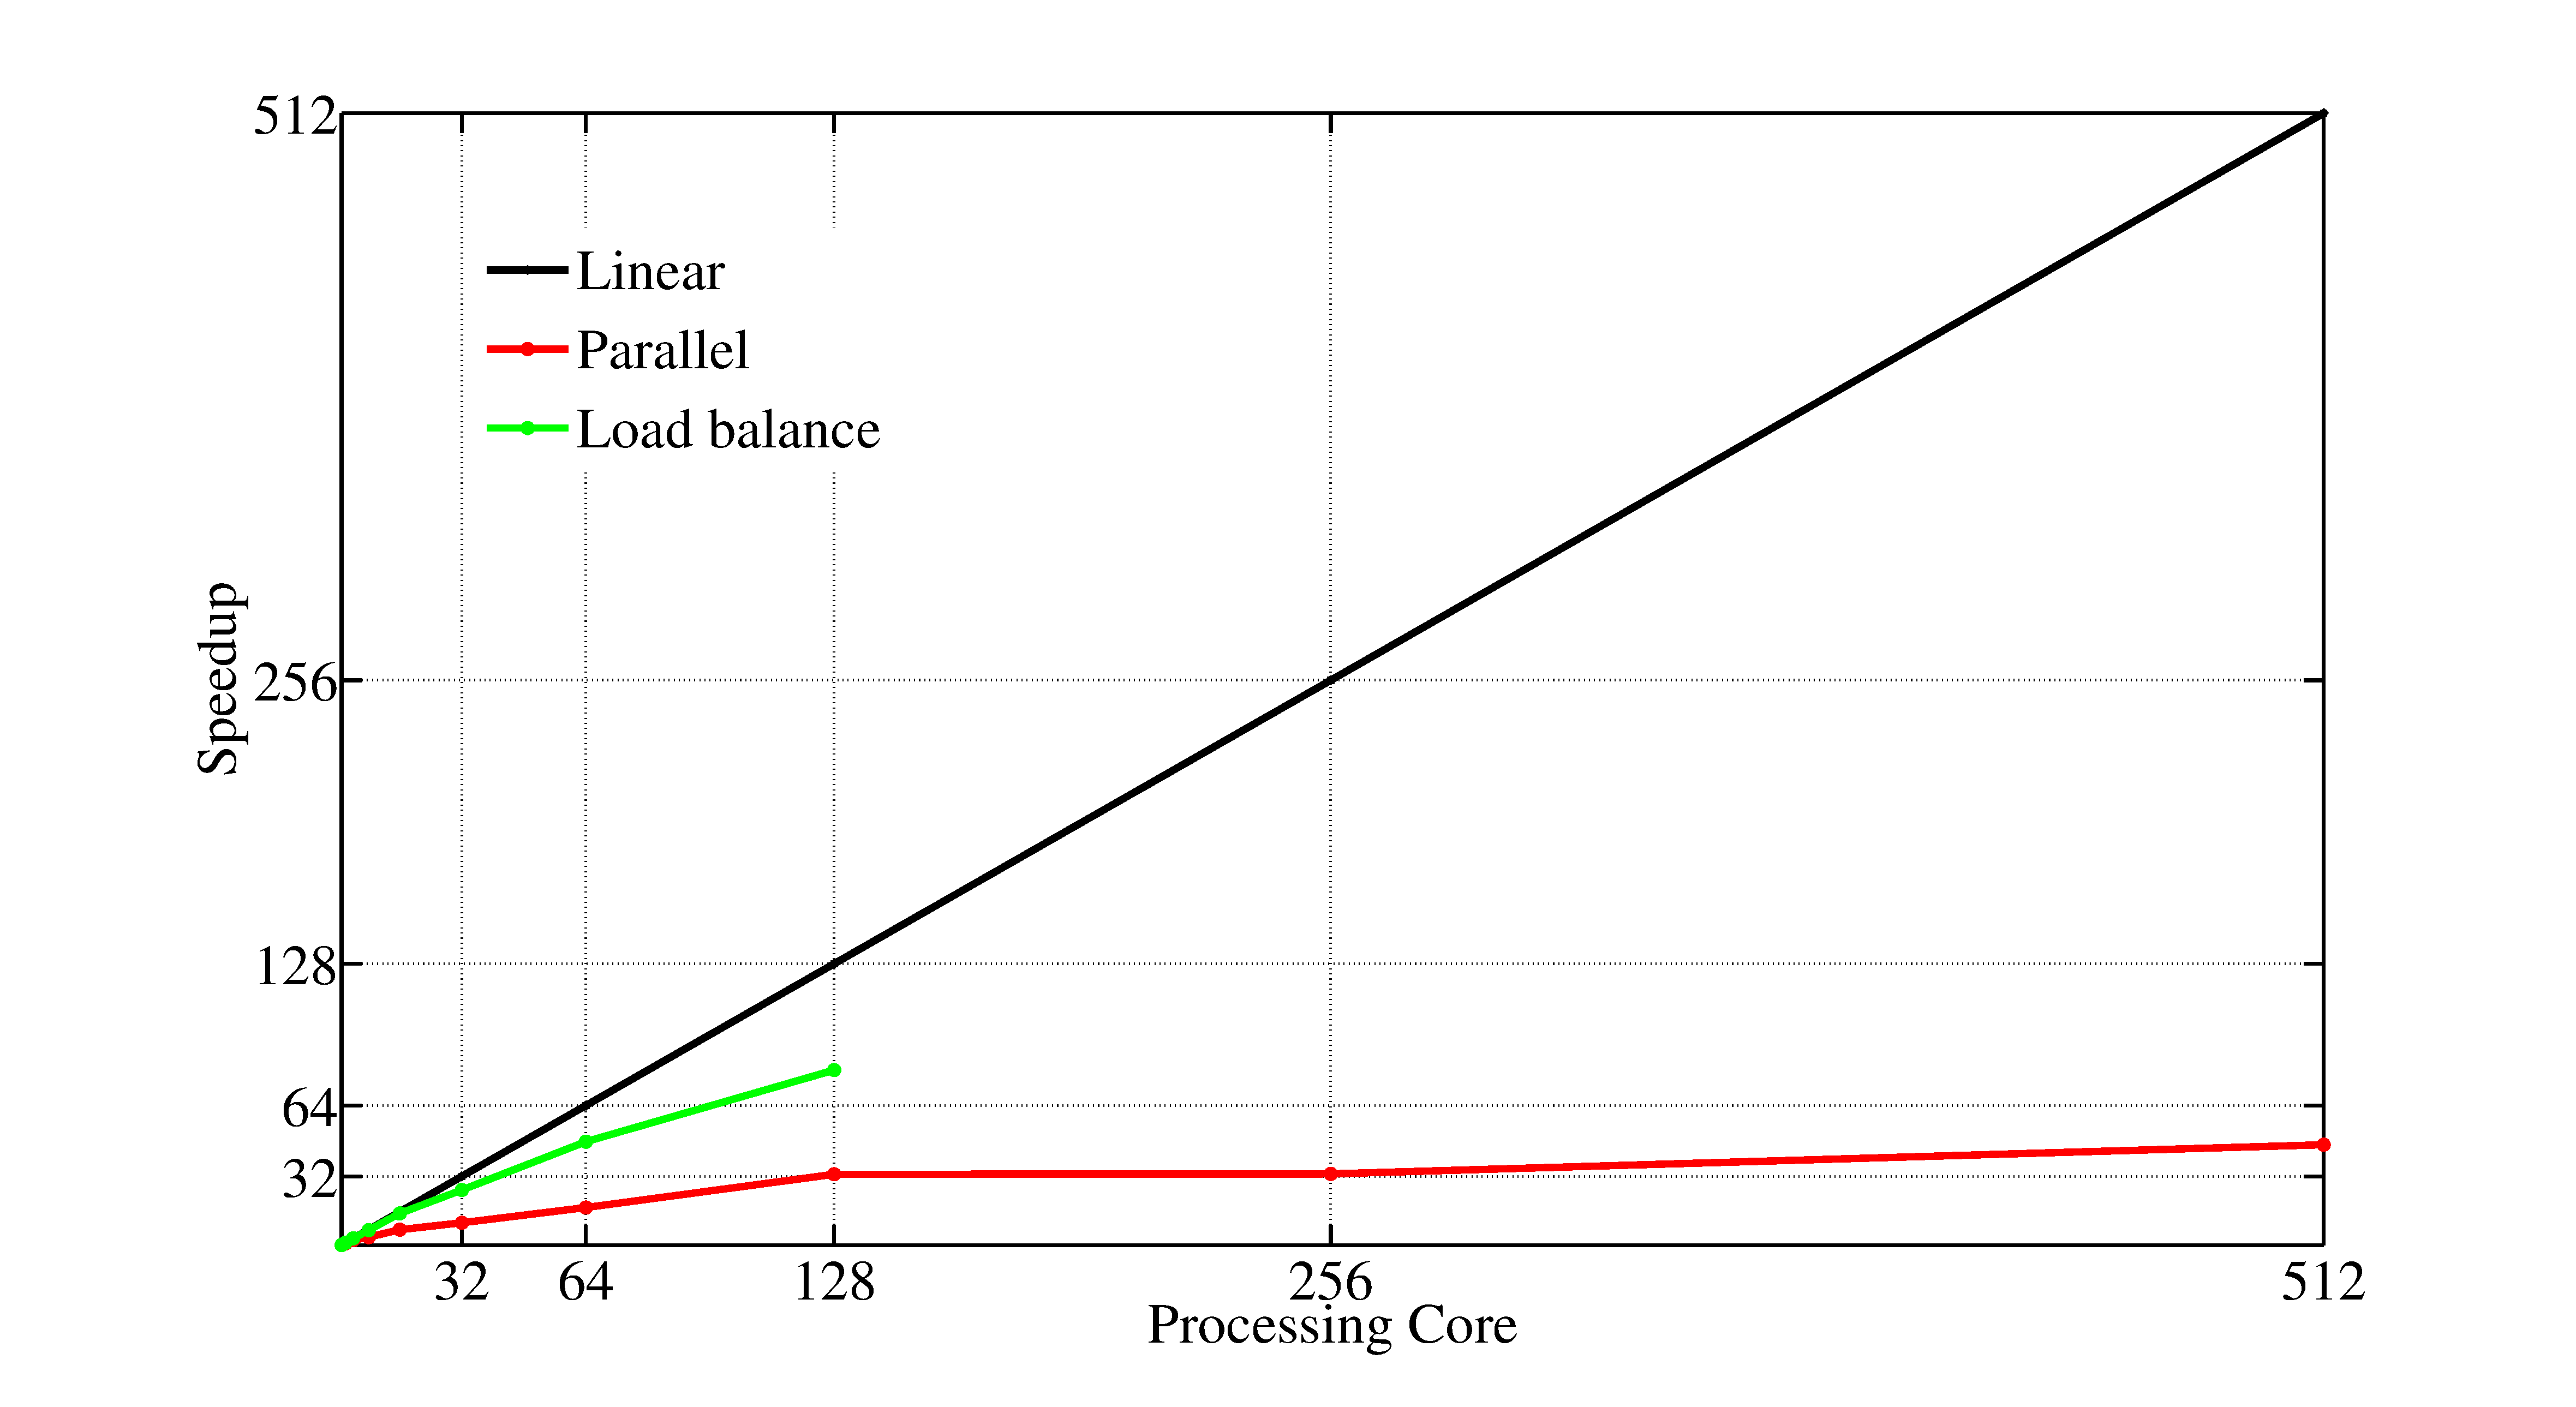
\includegraphics[width=40pc,trim=30 20 150 50, clip,]{figures/speedup.eps}
\caption{The same as Fig. \ref{timing} ,but for the parallel speedup}
\label{spd}
\end{figure}


\subsection{Tables}
%%%%%%%%%%%%%%%%%%%%%%%%%%%%%%%%%%%%%%%%%%%%%%%%%%%%%%%%%%%%%%%%%%%%%
% TABLES
%%%%%%%%%%%%%%%%%%%%%%%%%%%%%%%%%%%%%%%%%%%%%%%%%%%%%%%%%%%%%%%%%%%%%


%%%%%%%%%%%%%%%%%%%%%%%%%%%%%%%%%%%%%%%%%%%%%%%%%%%%%%%%%%%%%%%%%%%%%
% ACKNOWLEDGMENTS
%%%%%%%%%%%%%%%%%%%%%%%%%%%%%%%%%%%%%%%%%%%%%%%%%%%%%%%%%%%%%%%%%%%%%

\begin{acknowledgment}
The National Center for Atmospheric Research is sponsored by the National
Science Foundation.  This work is supported by ....
\end{acknowledgment}


%%%%%%%%%%%%%%%%%%%%%%%%%%%%%%%%%%%%%%%%%%%%%%%%%%%%%%%%%%%%%%%%%%%%%
% REFERENCES
%%%%%%%%%%%%%%%%%%%%%%%%%%%%%%%%%%%%%%%%%%%%%%%%%%%%%%%%%%%%%%%%%%%%%
% Create a bibliography directory and place your .bib file there.
\ifthenelse{\boolean{dc}}
{}
{\clearpage}
\bibliographystyle{ametsoc}
\bibliography{../bibliography/references}
%\bibliography{references}
\end{document}
%%%%%%%%%%%%%%%%%%%%%%%%%%%%%%%%%%%%%%%%%%%%%%%%%%%%%%%%%%%%%%%%%%%%%
% END OF TEMPLATE
%%%%%%%%%%%%%%%%%%%%%%%%%%%%%%%%%%%%%%%%%%%%%%%%%%%%%%%%%%%%%%%%%%%%%
